\section{The corridor in OpenStreetMap}
\label{sec:data}

\begin{figure*}[t]
\centering
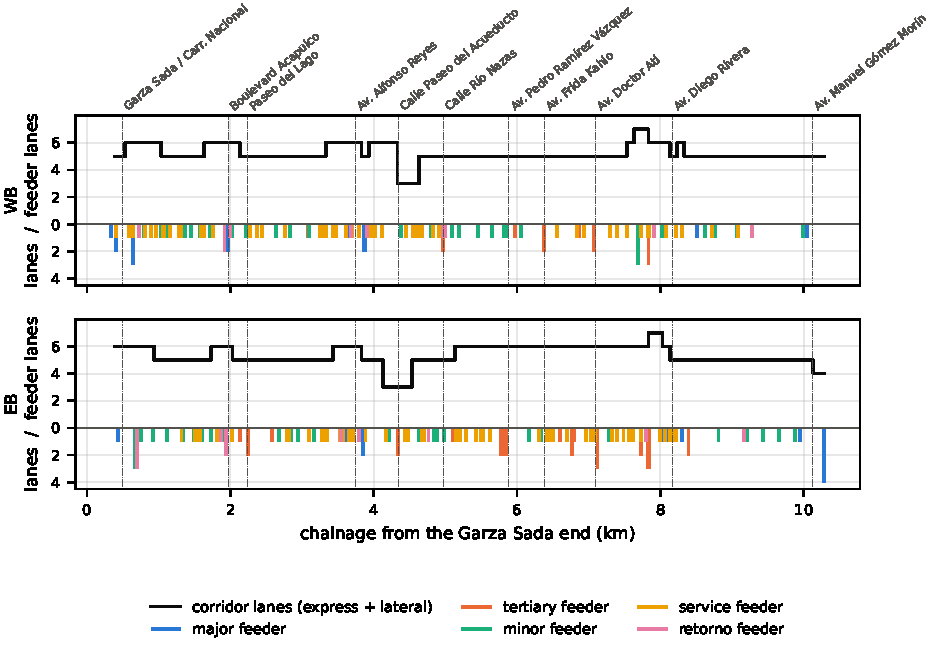
\includegraphics[width=\textwidth]{figures/inventory.pdf}
\caption{Inventory along the corridor, measured from the Garza Sada end
(top: westbound, towards San Pedro; bottom: eastbound). Black: corridor
lanes per direction (express plus frontage). Below the axis: every feeder
approach, with stem length equal to its lanes, coloured by road class.
Dotted lines mark the \InvJunctions\ junctions that split the corridor
into segments. Note the drop to three lanes at 4.4--4.6\,km.}
\label{fig:inventory}
\end{figure*}

\paragraph{Extraction.} We download the street network in 0.01-degree
tiles along the corridor from the OpenStreetMap API (the Overpass mirrors
were saturated on the day). The corridor consists of the \texttt{trunk}
(express) and \texttt{secondary}/\texttt{tertiary} (frontage) ways named
L\'azaro C\'ardenas that lie within 120\,m of the centre line. We assign
each one-way way to a direction by its travel direction along the
chainage. Every other street way that touches a corridor node is a
candidate feeder. One-way tags decide whether it can deliver vehicles
(an approach), receive them (a departure), or both. Chains of unnamed
links that only join the corridor to itself (express--frontage
transfers, U-turns, median crossings) are internal; we found
\InvInternalLinks\ such ways and removed them. A link that does reach the
outside takes the demand class of the most important road it reaches, so
a ramp that only leads to a parking aisle counts as a service access.

\paragraph{What feeds the avenue.} Over \InvLengthKm\,km we find
\InvApproaches\ approaches. \InvServiceApproaches\ of them are
\texttt{service} ways (driveways, plaza and parking entrances), and
\InvNRetorno\ are retornos (U-turns and median crossings that bring
vehicles from the opposite carriageway, \InvLanesRetorno\ lanes; each is
also an exit of the direction it leaves). The other
\InvApproachesNoService\ are streets: \InvNMajor\ major (trunk, primary,
secondary and their links), \InvNTertiary\ tertiary and \InvNMinor\
residential. Together the streets bring \InvFeederLanesNoService\ feeder
lanes (\InvFeederLanes\ including driveways). \InvTerminal\ approaches end
at the corridor (T-junctions, ramps); \InvCrossing\ cross it. The
cross-section is \InvExpressLanes\ express lanes plus two or three
frontage lanes, for a median of \InvMainlineLanes\ lanes per direction
(range \InvMainlineMin--\InvMainlineMax).

The conversation that motivated this project estimated
\LLMAccLo--\LLMAccHi\ accesses, \LLMLanesLo--\LLMLanesHi\ feeder lanes and
\LLMMainLo--\LLMMainHi\ lanes per direction, without giving sources. The
street counts land inside all three ranges. The lane ratio is real: about
\InvLaneRatioNoService:1 without driveways and \InvLaneRatio:1 with them.
The question is whether it means anything.

\paragraph{Data quality.} All corridor ways carry a \texttt{lanes} tag
(\InvCorridorTaggedPct\%). Only \InvTaggedPct\% of the feeder approaches
do; the rest take a class default (one lane per direction for
residential and service, two for tertiary). OpenStreetMap marks only
\InvSignalsOSM\ traffic signals on the corridor, all at Alfonso Reyes.
That is surely incomplete, so we also treat as signalised every frontage
junction fed by a major street or a tertiary street with at least two
lanes. This gives \InvSignalsWB\ signalised cells westbound and
\InvSignalsEB\ eastbound. The model's main bottleneck depends on one
mapped feature, and we test it directly (Section~\ref{sec:results}):
between 4.36 and 4.55\,km the frontage road merges into the express lanes
through a \texttt{secondary\_link} and reappears only after the stretch,
so the corridor narrows from five lanes to three between the Alfonso Reyes
overpass and the bridge over the Canal del Arroyo Seco.

\paragraph{One field estimate.} Alfonso Reyes reaches the corridor with
four lanes from the south. Two of them join L\'azaro C\'ardenas towards
San Pedro (westbound). While Alfonso Reyes has red, only one of them moves,
through a continuous turn; on green both move. An observer on site
estimated 7--10 vehicles per minute on red and 14--18 on green. Weighting
by the model's green share for the cross street gives
\FcWBLo--\FcWBHi\,veh/h for the whole junction (named street and its
unnamed ramps, retornos excluded). The demand model had assumed
\FcWBAssumed\,veh/h there, mostly from a two-lane slip ramp rated as a
major feeder. The count replaces the assumption: the base run uses the
middle of the range, the Monte Carlo draws inside it, and the
continuous-turn lane bypasses the signal. The count records what entered,
so it equals demand only if no queue remains on Alfonso Reyes after the
green; it is an estimate, not a measurement.
